\documentclass[13pt]{article}

\usepackage{microtype}
\usepackage{array}
\usepackage{amsmath}
\usepackage{graphicx}
\usepackage[english]{babel}
\usepackage{listings}
\usepackage{titling}
\usepackage[a4paper]{geometry}

\renewcommand{\baselinestretch}{1.5}
\renewcommand{\maketitlehooka}{\fontfamily{phv}\selectfont}

\geometry{includehead, includefoot, top=1.2cm, bottom=1.4cm, headheight=0cm}


% Er zijn talloze parameters ...
\lstset{language=C++, showstringspaces=false, basicstyle=\normalsize,
  numbers=left, numberstyle=\small, numberfirstline=false, breaklines=true,
  stepnumber=1, tabsize=8, 
  commentstyle=\ttfamily, identifierstyle=\ttfamily,
  stringstyle=\itshape}

\title{\vspace{-1.3cm} Verslag vierde programmeeropdracht}

\author{Alex Keizer \& L\'{e}on van Velzen}

\begin{document}

\maketitle
\section{Uitleg programma}

Dit programma stelt een gebruiker in staat om te rekenen met getallen waarvan de waarde extreem groot kan zijn. In veel programma's is de grootste waarde die een getal kan hebben gelijk aan de waarde dat nog representeerbaar is in 32 of 64 bits. De grootte van de getallen in dit programma zijn enkel gelimiteerd door de hoeveelheid geheugen van de computer. De gebruiker kan via een menu een drietal getallen manipuleren. De mogelijke operaties zijn: een getal invoeren, alle drie de getallen afdrukken, twee ervan optellen of vermenigvuldigen naar de derde, of een Fibonacci-getal in \'e\'en ervan laten uitrekenen. 

\section{Fibonacci}

De Fibonacci rij is als volgt gedefinieerd:

\begin{equation*}
    f(n) = \begin{cases}
               0               & n = 0\\
               1               & n = 1\\
               f(n-1) + f(n-2) & n > 1\\
           \end{cases}
\end{equation*}

De waardes in deze rij worden snel heel groot.

\begin{center}
    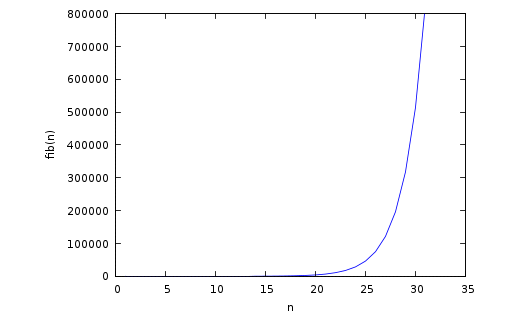
\includegraphics[scale=0.6]{graph.png}
\end{center}

Het is bewezen dat de groei van de rij van exponentiele orde is. Dankzij de gesloten vorm voor de Fibonacci rij $a_n={{\left(\sqrt{5}+1\right)^{n}+\left(1-\sqrt{5}\right)^{n}}\over{2^{n}}}$ is het bewijs hiervan simpel \cite{proof}.

\section{Tijd}

Tijd in uren besteed per week:

\begin{center}
\begin{tabular}{ |c|c|c| }
\hline
Week & Alex Keizer & L\'{e}on van Velzen \\
46 & 4 & 0 \\
47 & 0 & 6 \\
48 & 4 & 1 \\ 
\hline
Totaal & 8 & 7 \\
\hline
\end{tabular}
\end{center}

\begin{thebibliography}{9}
    \bibitem{proof} Prove Upper Bound (Big O) for Fibonacci's Sequence? Geraadpleegd op 2/12/2017, van https://math.stackexchange.com/q/674547
\end{thebibliography}

\section{Code}

\lstinputlisting{keizervanvelzen4.cpp}

\end{document}
